\chapter{Conexión y Compacidad}

\section{Conexión}

\begin{definicion}[Conexión]
    Decimos que un espacio topológico $(X,\T)$ es conexo si no existen dos abiertos disjuntos $U_1,U_2\in \T,~U_1\cap U_2=\emptyset$, tales que $X=U_1\cup U_2$; salvo el vacío y el total.

    En el caso de que un conjunto no sea conexo, diremos que es disconexo.

    Un conjunto $A\subset X$ es conexo si $(A,\T_A)$ es conexo. Es decir, cuando se habla de un subconjunto, implícitamente nos referimos a la topología inducida.
\end{definicion}

\begin{prop}[Caracterización de la Conexión]
    Sea $(X,\T)$ un espacio topológico. Entonces, las siguientes afirmaciones son equivalentes:
    \begin{enumerate}
        \item $(X,\T)$ es conexo.
        \item No existen dos cerrados disjuntos $C_1,C_2\subset C_{\T},~C_1\cap C_2=\emptyset$, tales que $X=C_1\cup C_2$; salvo el vacío y el total.
        \item Si $A\subset X$ es un conjunto abierto y cerrado, entonces $A=\emptyset$ o bien $A=X$.
        \item Toda aplicación continua $f:(X,\T)\to \left(\{0,1\},\T_{disc}\right)$ es constante.
    \end{enumerate}
\end{prop}
\begin{proof}\
    \begin{description}
        \item[$1)\Longrightarrow 2)$]
        Demostramos el contrarrecíproco. Supongamos que existen dos cerrados disjuntos $C_1,C_2\subset C_{\T},~C_1\cap C_2=\emptyset$, tales que $X=C_1\cup C_2$; con $C_1,C_2\neq \emptyset, X$.
        Entonces, sean $U_1=X\setminus C_1,~U_2=X\setminus C_2$. Tenemos que $U_1,U_2\in \T$, ya que $C_1,C_2\in C_{\T}$.
        Además, estos abiertos son disjuntos, ya que:
        $$U_1\cap U_2=X\setminus C_1 \cap X\setminus C_2 = X\setminus (C_1\cup C_2) = X\setminus X = \emptyset.$$
        Además, como $C_1,C_2\neq \emptyset, X$, entonces $U_1,U_2\neq X, \emptyset$.

        Por tanto, $(X,\T)$ es disconexo, por lo que queda demostrado el contrarrecíproco.

        \item [$2)\Longrightarrow 3)$] Sea $A$ un conjunto abierto y cerrado, y consideramos $C_1=A,~C_2=X\setminus A$. Tenemos que $C_1,C_2\in C_{\T}$, y $C_1\cap C_2=\emptyset$.
        Además, $X=C_1\cup C_2$. Por tanto, como $(X,\T)$ es conexo, $C_1=A=\emptyset$ o $C_1=A=X$.

        \item [$3)\Longrightarrow 1)$] Demostramos el contrarrecíproco. Supongamos que existen dos abiertos disjuntos $U_1,U_2\subset \T,~U_1\cap U_2=\emptyset$, tales que $X=U_1\cup U_2$; con $U_1,U_2\neq \emptyset, X$.
        Entonces, como $X=U_1\cup U_2$ y $U_1\cap U_2=\emptyset$, tenemos que $U_2=X\setminus U_1$, por lo que es cerrado. Por tanto, $U_2\neq \emptyset, X$ es abierto y cerrado a la vez, por lo que queda demostrado el contrarrecíproco.

        \item [$1)\Longrightarrow 4)$] Demostramos el contrarrecíproco.
        Si existe $f:(X,\T)\to \left(\{0,1\},\T_{disc}\right)$ continua y no constante, entonces definimos los siguientes conjuntos:
        \begin{equation*}
            U_1=f^{-1}(\{0\})\in \T
            \qquad
            U_2=f^{-1}(\{1\})\in \T
        \end{equation*}

        Tenemos que $U_1,U_2\notin \{\emptyset, X\}$ ya que no es constante; y se tiene que $U_1\cap U_2=\emptyset$, $U_1\cup U_2 = X$. Por tanto, $(X,\T)$ es disconexo, por lo que queda demostrado el contrarrecíproco.

        \item [$4)\Longrightarrow 1)$] Demostramos el contrarrecíproco. Como $X$ no es conexo, existen dos abiertos $U_1,U_2\in \T$, con $U_1,U_2\notin \{\emptyset, X\}$ tal que $U_1\cap U_2=\emptyset$, $U_1\cup U_2=X$.

        Entonces, definimos $f$ de la siguiente forma:
        \begin{equation*}
            f(x) = \left\{\begin{array}{ccl}
                0 & \text{si} & x\in U_1 \\
                1 & \text{si} & x\notin U_1 \Longleftrightarrow x\in U_2\Longleftrightarrow x\in X\setminus U_1 \\
            \end{array}\right.
        \end{equation*}

        Tenemos que $f$ no es constante, ya que ninguno de los conjuntos es el vacío. Además, $f$ es continua, ya que:
        \begin{equation*}
            f^{-1}(\emptyset)=\emptyset
            \qquad 
            f^{-1}(\{0,1\})=X
            \qquad 
            f^{-1}(\{0\})=U_1
            \qquad 
            f^{-1}(\{1\})=U_2
        \end{equation*}
        Por tanto, $f$ es continua, ya que la imagen inversa de todo abierto es un abierto; pero no es constante, por lo que queda demostrado el contrarrecíproco.
    \end{description}
\end{proof}



\begin{ejemplo}
    Veamos algunos ejemplos de conjuntos conexos:
    \begin{enumerate}
        \item $(X,\T_t)$ es conexo, ya que los únicos abiertos son el vacío y el total.

        \item Sea $X$ un conjunto tal que $|X|>1$. Entonces, $(X,\T_{disc})$ no es conexo, ya que fijado $x_0\in X$, entonces:
        \begin{equation*}
            X = (X\setminus \{x_0\})\cup \{x_0\}
        \end{equation*}

        \item $(X,\T_{CF})$. Si $X$ es finito, tenemos la topología discreta, por lo que no es conexo. Si $X$ es infinito, sí es conexo. Veámoslo:

        Sea $C\in \T_{CF}\cap C_{\T_{CF}}$, y supongamos que no es ni el vacío ni el total. Entonces, por ser cerrado es finito, y su complementario es también finito por ser abierto. Entonces, $X=C\cup (X\setminus C)$ es finito, por lo que llegamos a una contradicción. Por tanto, es conexo.

        \item Sea la hipérbola $H=\{(x,y)\in \bb{R}^2\mid xy=1\}$.

        Tenemos que $H$ no es conexo. Para verlo, sea $H^+$ el siguiente conjunto:
        \begin{equation*}
            H^+ = \{(x,y)\in \bb{R}^+\mid xy=1,~ x>0\}
        \end{equation*}

        Tenemos que:
        \begin{align*}
            H^+ &= H\cap (\bb{R}^+\times \bb{R}^+)\in {\T_u}_H\\
            H^+ &= H\cap (\bb{R}^+_0\times \bb{R}^+_0)\in C_{{\T_u}_H}
        \end{align*}

        Por tanto, $H^+$ es un abierto y cerrado. Como $H^+\neq \emptyset, H$, entonces $H$ no es conexo.
    \end{enumerate}
\end{ejemplo}

\begin{prop}
    Los conjuntos conexos de $(\bb{R}, \T_u)$ son exactamente los intervalos. Es decir, dado $A\subset \bb{R}$, tenemos que:
    \begin{equation*}
        A \text{ es conexo} \Longleftrightarrow A \text{ es un intervalo}
    \end{equation*}
\end{prop}
\begin{proof}
    Demostramos por doble implicación:
    \begin{description}
        \item[$\Longrightarrow)$] Sea $A$ conexo, y supongamos que no es un intervalo. Entonces, existen $a,b\in A$, $x\in X\setminus A$, tales que $a<x<b$. Entonces, consideramos los siguientes conjuntos:
        \begin{align*}
            U_1 &= A\cap ]-\infty, x[ \\
            U_2 &= A\cap ]x, \infty[
        \end{align*}

        Tenemos que $U_1,U_2\in {\T_u}_A$, ya que son intersecciones de abiertos de $\T_u$ con $A$.
        Además, $U_1\cap U_2=\emptyset$. Además, $U_1\cup U_2=A\setminus \{x\}=A$.

        Como $a\in U_1, b\notin U_1$, entonces $U_1\neq \emptyset, A$. Análogamente, se demuestra que $U_2\neq \emptyset, A$. Por tanto, $A$ es disconexo, llegando a una contradicción, por lo que $A$ es un intervalo.
        
        \item[$\Longleftarrow)$] Supongamos que $A\subset \bb{R}$ es un intervalo, y sea $f:(A,\T_A)\to \left(\{0,1\},\T_{disc}\right)$ continua. Tenemos que demostrar que $f$ es constante.
        
        Por el Teorema del Valor Intermedio visto en Cálculo I, tenemos que que $f(A)$ es un intervalo. Pero como $f(A)\subset \{0,1\}$, entonces $f(A)=\{0\}$ o bien $f(A)=\{1\}$, por lo que $f$ es constante.
    \end{description}
\end{proof}


\begin{teo}
    La imagen mediante una aplicación continua de un conexo es un conexo.
    
    Es decir, si $f:(X,\T)\to (Y,\T')$ es continua y $(X,\T)$ es conexo, entonces $f(X)$ es conexo.
\end{teo}
\begin{proof}
    Veamos el contrarrecíproco. Si $f(X)$ no fuese conexo, entonces por la caracterización de los conjuntos conexos, $\exists g:f(X)\to \left(\{0,1\},\T_{disc}\right)$ continua y no constante. Por tanto,
    \begin{equation*}
        g\circ f:(X,\T)\to \left(\{0,1\},\T_{disc}\right)
    \end{equation*}
    es continua (por ser composición de continuas) y no constante (ya que $g$ no lo es), por lo que $(X,\T)$ no es conexo, llegando a una contradicción.
\end{proof}

Como consecuencia inmediata, tenemos que si $f$ es un homeomorfismo, se trata de una doble implicación, ya que se puede considerar $f^{-1}$, también continua.
\begin{coro}
    La conexión es una propiedad topológica.\\Es decir, si $f:(X,\T)\to (Y,\T')$ es un homeomorfismo, entonces $f(X)=Y$ es conexo si y solo si $X$ es conexo.
\end{coro}

Para el caso de los espacios cocientes, tenemos el siguiente corolario:
\begin{prop}
    Sea $(X,\T)$ un espacio topológico, y sea $\cc{R}$ una relación de equivalencia en $X$. Consideramos $X/\cc{R}$ el espacio cociente con la topología cociente.
    Entonces:
    \begin{center}
        $X$ conexo $\Longrightarrow$ $X/\cc{R}$ conexo.
    \end{center}
\end{prop}
\begin{proof}
    Consideramos $p:(X,\T)\to (X/\cc{R}, \T/\cc{R})$ la proyección canónica en el cociente. Entonces, por el teorema anterior, como $p$ es continua, $p(X)$ es conexo. Pero como $p(X)=X/\cc{R}$ por ser $p$ sobreyectiva, entonces $X/\cc{R}$ es conexo.
\end{proof}

\begin{ejemplo}
    Veamos algunos resultados sobre el teorema anterior:
    \begin{enumerate}
        \item $(\bb{S}^1, {\T_u}_{\bb{S}^1})$ es conexo.

        Sabemos que $\bb{R}$ es conexo, por ser un intervalo. Nos definimos la siguiente aplicación:
        \Func{f}{(\bb{R}, \T_u)}{(\bb{S}^1, {\T_u}_{\bb{S}^1})}{x}{(\cos x, \sen x)}

        Tenemos que $f$ es continua y sobreyectiva, por lo que $f(\bb{R})=\bb{S}^1$ es conexo.

        \item $[a,b],~[a,b[, ~]a,b], ~]a,b[$ con $a<b$ no son homeomorfos.

        Supongamos que sí, lo son, por lo que existe el siguiente homeomorfismo:
        \begin{equation*}
            h:[a,b]\to [a,b[
        \end{equation*}

        Como $h$ es inyectiva, $h(a)$ o bien $h(b)$ no son $a$. Suponemos sin pérdida de generalidad que $h(b)\neq a$. Entonces:
        \begin{equation*}
            h_{\big| [a,b[}:[a,b[\longrightarrow [a,b[\setminus \{h(b)\}
        \end{equation*}
        es un homeomorfismo (luego continua). Pero $[a,b[$ es conexo y $[a,b[\setminus \{h(b)\}$ no lo es (no es un intervalo), por lo que llegamos a una contradicción.

        Para el resto de casos, se demuestra de forma análoga.

        \item $(\bb{R}, \T_u)$ no es homeomorfo a $(\bb{S}^1, {\T_u}_{\bb{S}^1})$.

        Supongamos que sí existe $h:\bb{R}\to \bb{S}^1$ homeomorfismo. Entonces, consideramos la siguiente restricción:
        \begin{equation*}
            h_{\big | \bb{R}\setminus \{0\}}: \bb{R}\setminus \{0\} \to \bb{S}^1\setminus \{h(0)\}
        \end{equation*}
        que también es un homeomorfismo. Como $\bb{S}^1\setminus \{h(0)\}$ es homeomorfo a $\bb{R}$, que es conexo, tenemos que $\bb{S}^1\setminus \{h(0)\}$ es conexo. No obstante, $\bb{R}\setminus \{0\}$ no lo es, por lo que llegamos a una contradicción.
    \end{enumerate}
\end{ejemplo}

\begin{coro}
    Sea un intervalo abierto $]a,b[\subset \bb{R}$, y sea $A\subset \bb{R}$. Entonces, Si $A$ es homeomorfo a $]a,b[$~, entonces $A$ es un intervalo abierto.
\end{coro}
\begin{proof}
    Si $A$ es homeomorfo a $]a,b[$, entonces $A$ debe ser conexo y así $A$ es un intervalo. Entonces, $A$ es uno de los siguientes tipos:
    \begin{align*}
        ]c,d[ &\quad -\infty \leq c<d\leq \infty\\
        [c,d[ &\quad -\infty < c<d\leq \infty \\
        ]c,d] &\quad -\infty \leq c<d< \infty \\
        [c,d] &\quad -\infty < c<d< \infty
    \end{align*}
    Por el apartado 2 del resultado anterior, tenemos que $A$ no es homeomorfo a los intervalos cerrados por uno o ambos extremos,
    por lo que:
    \begin{align*}
        A=]c,d[ &\quad -\infty \leq c<d\leq \infty \\& \hfill \qedhere
    \end{align*}
\end{proof}


Como consecuencia de lo visto, tenemos el siguiente resultado:
\begin{teo}[Invarianza del Dominio]
    Sean $A,B\subset \bb{R}$. Si $A,B$ son homeomorfos con la topología usual y $A$ es abierto, entonces $B$ es abierto.
\end{teo}
\begin{proof}
    Sea $h:A\to B$ un homeomorfismo entre ambos. Si $A\in \T_u$, como los intervalos son una base de la topología usual, entonces:
    \begin{equation*}
        A=\bigcup_{i\in I}~]c_i, d_i[ \text{\hspace{1cm} con } c_i<d_i,~ c_i,d_i\in \bb{R}
    \end{equation*}

    Entonces, la siguiente restricción es otro homomorfismo:
    \begin{equation*}
        h_{\big | ]c_i,d_i[}:]c_i,d_i[\to h(]c_i,d_i[)
    \end{equation*}

    Por consecuencia del corolario anterior, $h(]c_i,d_i[)$ es un intervalo abierto de $\bb{R}$, por lo que:
    \begin{equation*}
        B=h(A)=h\left(\bigcup_{i\in I}~]c_i, d_i[\right)=\bigcup_{i\in I} h(]c_i,d_i[)\in \T_u
    \end{equation*}
\end{proof}


\begin{teo}[del Valor Intermedio]
    Sea $f:(X,\T)\to (\bb{R}, \T_u)$ una aplicación continua con $(X,\T)$ conexo. Si existen $x_0,x_1\in X$ tales que $f(x_0)=a<b=f(x_1)$, entonces para todo $c\in ]a,b[$, existe $x\in X\mid f(x)=c$.
\end{teo}
\begin{proof}
    Supongamos que no existe $x\in X$ tal que $f(x)=c$.
    Entonces, $f(X)$ no es un intervalo, ya que $a < c < b$, con $a,b\in f(X)$ pero $c\notin f(X)$.
    Por tanto, $f(X)$ no es conexo, llegando a una contradicción.
\end{proof}


\begin{teo}[Borsuk-Ulam]
    Sea $f:(\bb{S}^n, {\T_u}_{\bb{S}^n})\to (\bb{R}, \T_u)$ una aplicación continua. Entonces, existe $p\in \bb{S}^n$ tal que $f(p)=f(-p)$.
\end{teo}
\begin{proof}
    Definimos la siguiente aplicación, que es continua por ser diferencia de continuas:
    \Func{g}{\bb{S}^n}{\bb{R}}{x}{f(x)-f(-x)}
    El teorema quedaría demostrado si encontramos $p\in \bb{S}^n$ tal que $g(p)=0$.
    
    Sea $q\in \bb{S}^n$. Si $g(q)=0$, $q$ es el valor buscado.
    En caso contrario, supongamos sin pérdida de generalidad que $g(q)>0$. Entonces,
    $-q\in \bb{S}^n$ y $$g(-q)=f(-q)-f(q)=-g(q)<0$$
    
    Por tanto, por el teorema del valor intermedio, como $g$ es continua y $\bb{S}^n$ es conexo (se demuestra más adelante, en el apartado \ref{ex:SnConexo} del ejemplo de la página \pageref{ex:SnConexo}), $\exists p\in \bb{S}^n$ tal que $g(p)=0$, es decir, $f(p)=f(-p)$.
\end{proof}

Actualmente, demostrar si un conjunto es conexo o no es una tarea complicada, ya que está definido de forna negativa (\emph{no existen...}).
Probar la no existencia suele ser complicado, por lo que proporcionamos una serie de criterios que nos permiten demostrar la conexión de un conjunto de forma más sencilla.
Este es el primer criterio, que trata la unión de conjuntos conexos:
\begin{prop}\label{prop:UnionConexos}
    Sea $(X,\T)$ un espacio topológico, y $\{A_i\}_{i\in I}$ una familia de conjuntos conexos con $A_i\subset X$ para todo $i\in I$.
    \begin{enumerate}
        \item Si $\bigcap\limits_{i\in I}A_i\neq \emptyset$, entonces $\bigcup\limits_{i\in I}A_i$ es conexo.
        \item Si existe $i_o\in I$ tal que $A_i\cap A_{i_0}\neq \emptyset~ \forall i\in I$, entonces $\bigcup\limits_{i\in I}A_i$ es conexo.
        \item Si la familia $A_i$ fuese numerable; es decir, podemos escribirla como $\{A_{i_n}\}_{n\in \bb{N}}$ (o cantidad finita) y se cumple que $A_{i_n}\cap A_{i_{n+1}}\neq \emptyset$, entonces $\bigcup\limits_{i\in I}A_i= \bigcup\limits_{n\in \bb{N}}A_{i_n}$ es conexo.
    \end{enumerate}
    % // TODO: Dibujos de las uniones
\end{prop}
\begin{proof} Demostramos cada una por separado:
    \begin{enumerate}
        \item Sea $f:\bigcup\limits_{i\in I}A_i \to (\{0,1\}, \T_{disc})$ continua. Tenemos que demostrar que es constante. Como cada $A_i$ es conexo, entonces:
        \begin{equation*}
            f_{\big |A_i}:A_i\to (\{0,1\}, \T_{disc})
        \end{equation*}
        es constante. Además, existe $x_0\in \bigcap\limits_{i\in I}A_i$, por lo que $f(x)=f(x_0)~ \forall x\in A_i$.
    
        Uniendo ambos resultados, tenemos que $f(x)=f(x_0)~\forall x\in \bigcup\limits_{i\in I}A_i$, por lo que $f$ es constante.

        \item Sea $f:\bigcup\limits_{i\in I}A_i \to (\{0,1\}, \T_{disc})$ continua. Tenemos que demostrar que es constante. Como cada $A_i$ es conexo, entonces:
        \begin{equation*}
            f_{\big |A_i}:A_i\to (\{0,1\}, \T_{disc})
        \end{equation*}
        es constante. En particular, $f_{\big |A_{i_0}}$ es constante. Sea $x_{i_0}\in A_{i_0}$.
        
        Para cada $i\in I$, $\exists x_i\in A_i\cap A_{i_0}$, por lo que $f(x_i)=f(x_{i_0})$.
        Por tanto, uniendo ambos resultados, tenemos que $f(x)=f(x_{i_0})~\forall x\in \bigcup\limits_{i\in I}A_i$, por lo que $f$ es constante.

        \item Definimos $Y_n = \bigcup\limits_{\substack{k\in \bb{N}\\k\leq n}}A_{i_k}$. Demostremos que $Y_n$ es conexo para todo $n\in \bb{N}$:        
        \begin{itemize}
            \item $n=1$. Es trivial, ya que $Y_1 = A_{i_1}$, que es conexo.
            \item Supuesto cierto para $n$, demostramos para $n+1$.
            
            Tenemos que $Y_{n+1}=Y_n\cup A_{i_{n+1}}$, ambos conexos. Además,
            \begin{equation*}
                Y_n \cap A_{i_{n+1}} = \left(\bigcup\limits_{\substack{k\in \bb{N}\\k\leq n}}A_{i_k}\right) \bigcap A_{i_{n+1}}
                = \bigcup\limits_{\substack{k\in \bb{N}\\k\leq n}}\left(A_{i_k} \cap A_{i_{n+1}}\right)
                \supset A_{i_{n}}\cap A_{i_{n+1}}\neq \emptyset
            \end{equation*}
            Por tanto, por el apartado 1 de esta proposición, $Y_{n+1}$ es conexo.
        \end{itemize}

        Como $\emptyset\neq A_{i_1}\subset \bigcap\limits_{n\in \bb{N}}Y_n$, entonces por el apartado 1 de esta proposición, $\bigcup\limits_{n\in \bb{N}}Y_n = \bigcup\limits_{n\in \bb{N}}A_{i_n}$ es conexo.
    \end{enumerate}
\end{proof}


\begin{teo}\label{teo:AdherenciaConexo}
    Sea $(X,\T)$ un espacio topológico, y $A\subset X$ un conjunto conexo. Entonces, para cualquier $B\subset X$ tal que $A\subset B\subset \ol{A}$ se tiene que $B$ es conexo.

    En particular, la adherencia de un conexo también es conexo.
\end{teo}
\begin{proof}
    Sea $f:B\to (\{0,1\},\T_{disc})$ continua. Tenemos que demostrar que $f$ es constante. Consideramos la restricción a $A$:
    \begin{equation*}
        f_{\big| A}: A \to (\{0,1\},\T_{disc})
    \end{equation*}
    Tenemos que dicha restricción es constante por ser $A$ conexo.
    Estudiamos ahora en $B\setminus A$.

    Sea $b\in B\setminus A$, y consideramos $\{f(b)\}\in \T_{disc}$. Por ser $f$ continua, también es continua en $b$,
    por lo que $\exists N\in N_b$ tal que $f(N)\subset \{f(b)\}$. Es decir, $f$ es constante en un entorno de $b$.

    Como $b\in B\setminus A \subset \ol{A}\setminus A$, entonces $b\in \partial A$. Por tanto, $\exists x\in A\cap N$. Como $f$ es constante en $N$, $f(x)=f(b)$. Además, como $x\in A$ y $f$ es constante en $A$, tenemos que $f(b)=f(x)$ para todo $x\in A$.

    Por tanto, $\forall b\in B\setminus A$, tenemos que $f(b)$ es constante e igual a $f(x)~\forall x\in A$.

    Por tanto, $f$ es constante en $B$, por lo que $B$ es conexo.
\end{proof}


Este criterio, relativo a los productos de conexos, nos será también de utilidad al trabajar con la topología producto:
\begin{prop}
    Sean $(X,\T), (Y,\T')$ dos espacios topológicos. Entonces, el producto $(X\times Y, \T\times \T')$ es conexo si y solo si $(X,\T), (Y,\T')$ son conexos.
\end{prop}
\begin{proof}
    Demostramos por doble implicación:
    \begin{description}
        \item[$\Longrightarrow)$]
        Si $X\times Y$ es conexo, como la proyección sobre $X$, $\pi_X:X\times Y\to X$ es continua y sobreyectiva, entonces $\pi_X(X\times Y)=X$ es conexo.

        Análogamente, se demuestra que $Y$ es conexo.

        \item[$\Longleftarrow)$] Veamos que $X\times Y$ es unión de conexos de forma que todos corten a uno fijo.

        Para cada $y\in Y$, consideramos los siguientes conjuntos:
        \begin{equation*}
            X_y = X\times \{y\},\qquad \text{con } y\in Y
        \end{equation*}
        Tenemos que $X_y$ es homeomorfo a $X$ para todo $y\in Y$, por lo que es conexo.

        Además, fijado $x_0\in X$, consideramos e siguiente conjunto homeomorfo a $Y$, luego conexo:
        \begin{equation*}
            Y_{x_0} = \{x_0\}\times Y
        \end{equation*}

        Por tanto, tenemos que $X\times Y = \bigcup\limits_{y\in Y}X_y = \left(\bigcup\limits_{y\in Y}X_y\right) \cup Y_{x_0}$, y la intersección $X_y\cap Y_{x_0}=\{(x_0,y)\}\neq \emptyset$ es no vacía para todo $y\in Y$.

        Por tanto, $X\times Y$ es conexo.
    \end{description}
\end{proof}

No obstante, incluso mostrar ejemplos de conjuntos conexos nos sigue resultando complicado. De hecho, con lo visto, no es fácil ver si $\bb{R}^n$ es conexo o no.
Para ello, introducimos los conceptos de conjunto estrellado y convexo.
\subsection{Conjuntos Estrellados y Convexidad}
En esta sección trataremos la Convexidad y los conjuntos estrellados. Aunque es cierto que tan solo nos serán de ayuda en caso de
espacios vectoriales reales, estos conceptos nos son de ayuda para trabajar con subconjuntos de $\bb{R}^n$, espacio vectorial real de gran importancia.

\begin{definicion}[Conjunto estrellado]
    Sea $V$ un espacio vectorial.
    Decimos que un conjunto $C\subset V$ es estrellado desde $x_0\in C$ si para todo $x\in C$, se cumple que el segmento que une $x$ con $x_0$, $[x,x_0]$, está en $C$. Es decir,
    \begin{equation*}
        (1-t)x + tx_0 \in C  \qquad \forall t\in [0,1],\forall x\in C
    \end{equation*}
    %// TODO: Dibujo conjunto estrellado. Estrella

    Decimos que un conjunto $C\subset \bb{R}^n$ es estrellado si es estrellado desde algún $x_0\in C$.
\end{definicion}
\begin{definicion}[Conjunto convexo]
    Sea $V$ un espacio vectorial.
    Decimos que un conjunto $C\subset V$ es convexo si es estrellado desde todos sus puntos. Es decir, para todo $x,y\in C$, el segmento que une $x$ con $y$, $[x,y]$, está en $C$. Es decir,
    \begin{equation*}
        (1-t)x + ty \in C  \qquad \forall t\in [0,1],\forall x,y\in C
    \end{equation*}
    %// TODO: Dibujo conjunto convexo
\end{definicion}
Como consecuencia inmediata de las definiciones, tenemos que todo conjunto convexo es estrellado. No obstante, no es cierto que todo conjunto estrellado sea convexo, como se puede ver en el siguiente ejemplo:
% // TODO: Dibujo conjunto estrellado no convexo
\begin{lema}
    Sea $E$ un espacio vectorial, y $C\subset V$ un subconjunto suyo.
    \begin{center}
        $C$ es convexo $\Longrightarrow$ $C$ es estrellado.
    \end{center}
\end{lema}

\begin{ejemplo}
    Veamos algunos ejemplos de conjuntos estrellados y convexos:
    \begin{enumerate}
        \item $\bb{R}^n$ es evidentemente convexo.
        \item La semirrecta con inicio en el origen que pasa por $x$, $S_x = \{\lm x \mid \lm > 0\}$, es convexo.
        
        En efecto, dado $x_0\in S_x$, entonces $x_0=\lm x$, con $\lm > 0$. Entonces, para todo $t\in [0,1]$:
        $$(1-t)x+tx_0=(1-t)x+t\lm x=(1-t+t\lm)x\in S_x \Longrightarrow
        1-t+t\lm > 0$$
        que, como $t\in [0,1]$, se cumple.
        
        Por tanto, $S_x$ es estrellado desde $x_0$. Como $x_0$ es arbitrario, $S_x$ es convexo.
    \end{enumerate}
\end{ejemplo}

\begin{prop}
    Sea $V$ un espacio vectorial normado, y $C\subset V$ un subconjunto suyo.
    \begin{center}
        $C$ es estrellado $\Longrightarrow$ $C$ es conexo.
    \end{center}
\end{prop}
\begin{proof} 
    Cada segmento cerrado uniendo dos puntos $x,x_0\in V$ es un conjunto conexo, ya que son la imagen de la siguiente aplicación:
    \Func{f}{[0,1]}{V}{t}{(1-t)x+tx_0}
    que es continua, (de hecho, es lipschitziana):
    \begin{equation*}
        \|f(t)-f(t')\|=\|(1-t)x+tx_0-(1-t')x-t'x_0\|=\|(t'-t)(x-x_0)\|=\|x-x_0\||t-t'|
    \end{equation*}
    Por el ejercicio \ref{ej:Tema2.1}, como $f$ es lipschitziana, entonces es continua. Además, como $[0,1]$ es conexo, entonces todos los segmentos dichos son conexos.

    Entonces, como $C$ es estrellado, supongamos que lo es desde $x_0\in C$:
    \begin{equation*}
        C = \bigcup_{x\in C}\{x\} \subset \bigcup_{x\in C}[x,x_0] \stackrel{(\ast)}{\subset} C
    \end{equation*}
    donde en $(\ast)$ hemos usado que $C$ es estrellado. Por tanto, como $x_0\in \bigcap\limits_{x\in C}[x,x_0]$, por el primer apartado del resultado anterior tenemos que $C$ es conexo.
\end{proof}
\begin{coro}
    Sea $V$ un espacio vectorial normado, y $C\subset V$ un subconjunto suyo.
    \begin{center}
        $C$ es convexo $\Longrightarrow$ $C$ es conexo.
    \end{center}
\end{coro}
\begin{proof}
    Como $C$ es convexo, entonces es estrellado, por lo que por la proposición anterior, $C$ es conexo.
\end{proof}

Una vez visto este nuevo criterio, podemos introducir nuevos ejemplos de conjuntos conexos:
\begin{ejemplo}
    Otros ejemplos de conjuntos conexos son:
    \begin{enumerate}
        \item $\bb{R}^n$ es conexo por ser estrellado.
        \item \label{ex:SnConexo}
        La esfera $\bb{S}^n$ es conexo con la ${\T_u}_{\bb{S}^n}$.

        Tenemos que:
        \begin{equation*}
            \bb{S}^n=(\bb{S}^n\setminus \{N\}) \cup (\bb{S}^n\setminus \{S\})
        \end{equation*}
    
        Ambos conjuntos son conexos por ser homeomorfos a $\bb{R}^n$, y su intersección es no vacía. Por tanto, $\bb{S}^n$ es conexo.

        \item $\bb{R}^n \setminus \{0\}$ es conexo para $n\geq 2$.

        Podemos ver $\bb{R}^n\setminus \{0\}$ como la unión de $\bb{S}^{n-1}$ con todas las semirrectas $S_x$ para cada $x\in \bb{S}^{n-1}$. La esfera tenemos que es conexa, y las semirrectas $S_x$ son estrellados, luego conexos.

        Como cada $S_x\cap \bb{S}^{n-1}=\{x\}\neq \emptyset$, entonces $\left(\bigcup\limits_{x\in \bb{S}^{n-1}}S_x\right)\cup \bb{S}^{n-1}=\bb{R}\setminus \{0\}$ es conexo.

        \item Sea $(X,\T)$ un espacio vectorial normado. Entonces, las bolas abiertas son conjuntos conexos.
        
        Demostramos en primer lugar que son convexos. Sea $x_0\in X,~r\in \bb{R}^+$. Entonces, para todo $x,y\in B(x_0,r)$, tenemos que:
        \begin{multline*}
            \|(1-t)x + ty- x_0\| = \|(1-t)(x-x_0) + t(y-x_0)\| \leq \\ \leq (1-t)\|x-x_0\| + t\|y-x_0\| < (1-t)r + tr = r
        \end{multline*}

        por tanto, son conjuntos convexos. Como $X$ es un espacio vectorial normado, son conexos.

        \item Sea $(X,\T)$ un espacio vectorial normado. Entonces, las bolas cerradas son conjuntos conexos.
    \end{enumerate}

    Ejemplos de conjuntos producto que son conexos son:
    \begin{enumerate}
        \item El cilindro $\bb{S}^1\times \bb{R}=\{(x,y,z)\in \bb{R}^3\mid x^2 + y^2=1\}$ es conexo por ser producto de conexos.

        \item El toro es conexo por ser homeomorfo a $(\bb{S}^1\times \bb{S}^1)/\cc{R}$, y este lo es por serlo $\bb{S}^1\times \bb{S}^1$, que es producto de conexos.

        \item El espacio proyectivo es también conexo, por serlo $\bb{R}^n\setminus \{0\}$ con $n\geq 2$.
    \end{enumerate}
\end{ejemplo}
Notemos entonces que, auque estas propiedades no sean topológicas, sino algebraicas, nos permiten demostrar la conexión de conjuntos de forma sencilla.
Por último, en el Teorema \ref{prop:UnionConexos} se ha tratado la unión de conjuntos conexos, aunque en ningún momento se ha tratado la intersección de conjuntos conexos.
Esto es más complejo, pero tenemos el siguiente resultado que también nos será de ayuda:
\begin{prop}
    Sea $V$ un espacio vectorial, y sean $A,B\subset V$ dos subconjuntos suyos.
    \begin{center}
        $A,B$ convexos $\Longrightarrow$ $A\cap B$ convexo.
    \end{center}
\end{prop}
\begin{proof}
    Sean $x,y\in A\cap B$. Entonces, como $A$ es convexo, $[x,y]\subset A$. Análogamente, $[x,y]\subset B$. Por tanto, $[x,y]\subset A\cap B$, por lo que $A\cap B$ es convexo.
\end{proof}

\subsection{Componentes Conexas}
\begin{definicion}
    Sea $(X,\T)$ un espacio topológico, y consideramos $x_0\in X$. Llamamos componente conexa de $x_0$ al siguiente conjunto:
    \begin{equation*}
        C(x_0) = \bigcup\{A\subset X\mid x_0\in A,~A\text{ es conexo}\}
    \end{equation*}
\end{definicion}

\begin{prop}
    Sea $(X,\T)$ un espacio topológico, y $x_0\in X$. Entonces, la componente conexa $C(x_0)$ de $x_0$ es el mayor conexo que contiene a $x_0$.
\end{prop}
\begin{proof}
    Veamos en primer lugar que $C(x_0)$ es conexo. Tenemos que es la unión de conexos, y su intersección es no vacía,
    ya que $$x_0\in \bigcap\{A\subset X\mid x_0\in A,~A\text{ es conexo}\}$$
    Por tanto, $C(x_0)$ es conexo.

    Además, sea $C$ un conexo que contiene a $x_0$. Entonces, de forma directa se tiene que $C\subset C(x_0)$.
\end{proof}

\begin{ejemplo}
    Veamos algunos ejemplos de componentes conexas:
    \begin{enumerate}
        \item En $\bb{R}\setminus \{0\}$, tenemos que $C(1)=\bb{R}^+$.
        \item En $\bb{Q}$, tenemos que $C(1)=\{1\}$.
    \end{enumerate}
\end{ejemplo}

\begin{prop} \label{prop:PropiedadesComponentesConexas}
    Sea $(X,\T)$ un espacio topológico. Entonces, se tiene las siguientes propiedades:
    \begin{enumerate}
        \item Las componentes conexas de un espacio topológico $(X,\T)$ dan una partición de $X$.
        \item Un espacio topológico $(X,\T)$ es conexo si y solo si tiene una única componente conexa.
        \item Las componentes conexas de $(X,\T)$ son cerrados de $(X,\T)$.
    \end{enumerate}
\end{prop}
\begin{proof} Vemos cada propiedad por separado:
    \begin{enumerate}
        \item Tomamos dos puntos distintos $x,y\in X$. Veamos que $C(x)=C(y)$ o bien $C(x)\cap C(y)=\emptyset$.

        Supongamos que $C(x)\cap C(y)\neq \emptyset$. Entonces, $C(x)\cup C(y)$ es conexo, por ser unión de dos conexos con intersección no vacía. Por tanto,
        \begin{equation*}
            x\in C(x)\subset C(x)\cup C(y) \stackrel{(\ast)}{\subset} C(x)
        \end{equation*}
        donde en $(\ast)$ se ha aplicado que $C(x)$ es el mayor conexo que contiene a $x$. Por tanto, $C(x)=C(x)\cup C(y)$. Análogamente, se demuestra el mismo resultado para $C(y)$, es decir, $C(y)=C(x)\cup C(y)$. Por tanto, $C(x)=C(y)$.
        
        Por tanto, vemos que dos componentes conexas son disjuntas o iguales. Si demostramos que la unión de todas las componentes conexas es $X$, entonces tenemos que las componentes conexas dan una partición de $X$.
        Es claro que:
        \begin{equation*}
            X=\bigcup_{x\in X}\{x\} \subset \bigcup_{x\in X}C(x)\subset X \Longrightarrow X=\bigcup_{x\in X}C(x)
        \end{equation*}
        Por tanto, las componentes conexas dan una partición de $X$.

        \item Demostramos por doble implicación:
        \begin{description}
            \item[$\Longrightarrow)$] Supongamos que $X$ es conexo. Entonces, $\exists x_0\in X$ tal que $X=C(x_0)$. Por tanto, como las componentes conexas dan una partición de $X$, $C(x_0)$ es la única componente conexa de $X$.
            \item[$\Longleftarrow)$] Supongamos que $X$ tiene una única componente conexa. Entonces, como las componentes conexas dan una partición de $X$, $X=C(x_0)$ para algún $x_0\in X$. Por tanto, como $C(x_0)$ es conexo, $X$ también lo es.
        \end{description}

        \item Si $C(x)$ es la componente conexa de $x\in X$, sabemos que $\ol{C(x)}$ es un conexo. Pero:
        \begin{equation*}
            x\in C(x)\subset \ol{C(x)} \stackrel{(\ast)}{\subset} C(x)
        \end{equation*}
        donde en $(\ast)$ hemos aplicado que $C(x)$ es el mayor conexo que contiene a $x$. Entonces, $C(x)=\ol{C(x)}$, por lo que $C(x)$ es cerrado.
    \end{enumerate}
\end{proof}

La siguiente propiedad nos da una condición suficiente para que una partición por conexos coincida con las componentes conexas:
\begin{prop}\label{prop:ParticionConexosAbiertos}
    Sea $(X,\T)$ un espacio topológico, y $\{A_i\}_{i\in I}$ una partición de $X$ donde cada $A_i\in \T$ y es conexo. Entonces la familia ${\{A_i\}}_{i\in I}$ es el conjunto de todas las componentes conexas de $(X,\T)$.
\end{prop}
\begin{proof}
    Sea $x\in X$ e $i_0\in I$ tal que $x\in A_{i_0}$. Veamos que $C(x)=A_{i_0}$.
    \begin{description}
        \item[$\supset)$] Como $A_{i_0}$ es conexo y $x\in A_{i_0}$, entonces $A_{i_0}\subset C(x)$.
        \item[$\subset)$] Supongamos que $C(x)\setminus A_{i_0}\neq \emptyset$. Entonces:
        \begin{align*}
            C(x) &= (C(x)\cap A_{i_0}) \bigcup \left(C(x)\cap (X\setminus A_{i_0})\right) =\\
            &= (C(x)\cap A_{i_0}) \bigcup \left(C(x)\cap \bigcup_{i\in I\setminus \{i_0\}}A_i\right)
        \end{align*}
        Por tanto, $C(x)$ se expresa como unión de dos abiertos de $\T_{C(x)}$, disjuntos y no vacíos, por lo que $C(x)$ no es conexo, llegando a una contradicción.
        
        Por tanto, $C(x)\setminus A_{i_0}=\emptyset$, por lo que $C(x)\subset A_{i_0}$.
    \end{description}
\end{proof}

No obstante, se trata de una condición suficiente, pero no necesaria. Es decir, puede haber componentes conexas que no sean abiertas. Veamos un ejemplo:
\begin{ejemplo}
    Sea $X=\bb{R}\setminus \left\{\dfrac{1}{n}\mid n\in \bb{N}\right\}$.

    Tenemos que las componentes conexas de $X$ son:
    \begin{equation*}
        ]-\infty, 0] \qquad ]1,\infty[ \qquad \left]\dfrac{1}{n+1}, \dfrac{1}{n}\right[~~n\in \bb{N}
    \end{equation*}
    
    No obstante, $]-\infty, 0]$ no es abierto, ya que el $0$ no es interior. Esto se debe a que
    $\nexists \veps\in \bb{R}^+$ tal que $]-\veps, \veps[\cap X \subset ]-\infty, 0]$, ya que $]-\veps, \veps[\cap X$ contiene elementos positivos.
\end{ejemplo}

Ya que toda aplicación continua lleva conjuntos conexos en conexos, concluimos el siguiente resultado:
\begin{prop}
    Sea $f:(X,\T)\to (Y,\T')$ una aplicación continua y sea $x\in X$:
    \begin{enumerate}
        \item $f(C(x))\subset C(f(x))$.
        \item Si $f$ es un homeomorfismo, entonces $f(C(x))=C(f(x))$.
    \end{enumerate}
\end{prop}
\begin{proof}
    Demostramos cada apartado por separado:
    \begin{enumerate}
        \item Como $C_(x)$ es conexo, entonces $f(C(x))$ es conexo, por ser $f$ continua.
        Además, como $x\in C(x)$, $f(x)\in f(C(x))$ conexo, por lo que $f(C(x))\subset C(f(x))$ por ser $C(f(x))$ el mayor conexo que contiene a $f(x)$.
        \item Como $f$ es un homeomorfismo, entonces $f^{-1}$ es continua. Consideramos $y\in C(f(x))$. Entonces, por ser $f$ biyectiva, $\exists!~x\in X$ tal que $f(x)=y$. Entonces:
        \begin{equation*}
            f^{-1}(C(f(x))) \subset C(f^{-1}(f(x))) = C(x) \Longrightarrow C(f(x)) \subset f(C(x))
        \end{equation*}
    \end{enumerate}
\end{proof}
\begin{coro}
    El número de componentes conexas es una propiedad topológica.

    Es decir, si $(X,\T)$ y $(Y,\T')$ son homeomorfos, entonces tienen el mismo número de componentes conexas.
\end{coro}


\section{Compacidad}

\begin{definicion}
    Sea $(X,\T)$ un espacio topológico. Decimos que $X$ es compacto si todo recubrimiento de $X$ por abiertos tiene un subrecubrimiento finito.
    Es decir, si $X=\bigcup\limits_{i\in I}U_i$ con $U_i\in \T$ para todo $i\in I$, entonces $\exists I_0\subset I$ \ul{finito} tal que $X=\bigcup\limits_{i\in I_0}U_i$.

    Un conjunto $A\subset X$ es compacto si $(A,\T_{A})$ es compacto.
\end{definicion}

\begin{ejemplo}
    Veamos algunos ejemplos de compactos:
    \begin{enumerate}
        \item $(\bb{R}^n,\T_u)$ no es compacto.
        
        Para verlo, un recubrimiento $\{U_n\}_{n\in \bb{N}}$ de $\bb{R}^n$ por abiertos es:
        \begin{equation*}
            U_n = B(0, n)  \qquad \forall n\in \bb{N}
        \end{equation*}

        Supongamos que existe un conjunto $N_0\subset \bb{N}$ finito tal que $\{U_n\}_{n\in N_0}$ es un recubrimiento de $\bb{R}^n$.
        Como $N_0$ es finito, $\exists n_0=\max N_0$, y se tiene que:
        \begin{equation*}
            \bb{R}^n= \bigcup_{n\in N_0}U_n = \bigcup_{n\in N_0}B(0,n) \subset B(0,n_0) \Longrightarrow \bb{R}^n \subset B(0,n_0)
        \end{equation*}
        que es un absurdo, ya que $\bb{R}^n$ no está acotado.

        \item $(X,\T_t)$ es compacto, ya que tan solo hay dos abiertos.
        
        \item Sea $(X,\T)$. Si $\T$ es finito, entonces $(X,\T)$ es compacto.
        
        \item $(X,\T_{disc})$ es compacto si y solo si $X$ es finito.
        \begin{description}
            \item[$\Longleftarrow)$] Si $X$ es finito, entonces $\T_{disc}$ es finito, por lo que $(X,\T_{disc})$ es compacto.
            \item[$\Longrightarrow)$] Demostramos el contrarrecíproco. Supongamos que $X$ es infinito. Entonces, $\{x\}_{x\in X}$ es un recubrimiento de $X$ por abiertos,
            pero no tiene ningún subrecubrimiento finito, ya que cada $x\in X$ está en un único abierto.
        \end{description}

        \item $(X,\T_{CF})$ es compacto.
        
        Sea $\{U_i\}_{i\in I}$ un recubrimiento de $X$ por abiertos, y elegimos $i_0\in I$ de forma que $U_{i_0}\neq \emptyset$.
        Entonces, $X\setminus U_{i_0}$ es finito, por lo que $\exists x_1,\dots,x_n\in X$ tal que $X\setminus U_{i_0}=\{x_1,\dots,x_n\}$.

        Para cada $j\in \{1,\dots,n\}$, consideramos $x_j$. Como $\{U_i\}_{i\in I}$ es un recubrimiento de $X$, entonces $\exists i_j\in I$ tal que $x_j\in U_{i_j}$.
        Por tanto, tenemos que el subrecubrimiento finito es:
        \begin{equation*}
            \{U_{i_0}\} \cup \{U_{i_j}\}_{j=1,\dots,n}
        \end{equation*}
    \end{enumerate}
\end{ejemplo}

\begin{prop}[Caracterización de la Compacidad]
    Sea $(X,\T)$ un espacio topológico y $\cc{B}$ una base de $\T$. Entonces, equivalen:
    \begin{enumerate}
        \item $X$ es compacto.
        \item Para cualquier familia de cerrados $\{F_i\}_{i\in I}$ de $X$ tal que $\bigcap\limits_{i\in I}F_i=\emptyset$,
        entonces $\exists n\in \bb{N}$ finito tal que $\bigcap\limits_{i=1}^n F_j=\emptyset$.
        \item Para cualquier recubrimiento de $X$ por abiertos básicos $\{B_i\}_{i\in I}$, con $B_i\in \cc{B}$ para todo $i\in I$,
        entonces $I_0\subset I$ finito tal que $X=\bigcup\limits_{i\in I_0} B_i$.
    \end{enumerate}
\end{prop}
\begin{proof} Demostramos mediante implicaciones dobles:
    \begin{description}
        \item[$1)\Longrightarrow 2)$] Supongamos que $X$ es compacto, y sea $\{F_i\}_{i\in I}$ una familia de cerrados de $X$ tal que $\bigcap\limits_{i\in I}F_i=\emptyset$.
        Consideramos $U_i=X\setminus F_i$, y tenemos que $\{U_i\}_{i\in I}$ es una familia de abiertos de $X$. Veamos que es un recubrimiento de $X$:
        \begin{equation*}
            X=X\setminus \bigcap_{i\in I}F_i = \bigcup_{i\in I}(X\setminus F_i) = \bigcup_{i\in I}U_i
        \end{equation*}

        Por tanto, como $X$ es compacto, entonces $\exists n\in \bb{N}$ tal que $X=\bigcup\limits_{i=1}^n U_i$. Entonces:
        \begin{equation*}
            X = \bigcup_{i=1}^n U_i = \bigcup_{i=1}^n (X\setminus F_i) = X\setminus \bigcap_{i=1}^n F_i \Longrightarrow \bigcap_{i=1}^n F_i = \emptyset
        \end{equation*}

        \item[$2)\Longrightarrow 1)$] Sea $\{U_i\}_{i\in I}$ un recubrimiento de $X$ por abiertos. Entonces, $\{X\setminus U_i\}_{i\in I}$ es una familia de cerrados de $X$ cuya intersección es nula.
        Por tanto, por hipótesis, $\exists n\in \bb{N}$ tal que $\bigcap\limits_{i=1}^n (X\setminus U_i)=\emptyset$. Entonces:
        \begin{equation*}
            \emptyset = \bigcap_{i=1}^n (X\setminus U_i) = X\setminus \bigcup_{i=1}^n U_i \Longrightarrow X \subset \bigcup_{i=1}^n U_i \subset X
        \end{equation*}
        Por doble inclusión, $X=\bigcup\limits_{i=1}^n U_i$, por lo que $X$ es compacto.

        \item[$1)\Longrightarrow 3)$] Como los abiertos básicos son abiertos, entonces se tiene de forma directa.
        
        \item[$3)\Longrightarrow 1)$] Sea $\{U_i\}_{i\in I}$ un recubrimiento de $X$ por abiertos. Por la definición de base, para cada $i\in I$, existe un
        conjunto de índices $J_i$ tal que $U_i=\bigcup\limits_{j\in J_i}B^i_j$ con $B^i_j\in \cc{B}$. Por tanto,
        \begin{equation*}
            X = \bigcup_{i\in I} U_i = \bigcup_{i\in I} \bigcup_{j\in J_i} B^i_j
        \end{equation*}
        Por tanto, por hipótesis $\exists I_0\subset I$ finito y, para cada $i\in I_0$, existe $J^0_i\subset J_i$ finito tal que:
        \begin{equation*}
            X = \bigcup_{i\in I_0} \bigcup_{j\in J^0_i} B^i_j
        \end{equation*}
        Como $I_0$ es finito y también lo son los $J^0_i$, entonces $\bigcup\limits_{j\in J^0_i} B^i_j$ es finito. Por tanto, $X$ es compacto.
    \end{description}
\end{proof}

En la definición de espacio compacto, se ha visto que un subconjunto es compacto si lo es con la topología inducida.
No obstante, la siguiente caracterización nos es de ayuda, ya que nos permite saber si un conjunto es compacto trabajando con los abiertos de la topología original.
\begin{prop}
    Sea $(X,\T)$ un espacio topológico y $A\subset X$.
    Entonces, $A$ es compacto si y solo si todo recubrimiento de $A$ por abiertos \ul{de $(X,\T)$} tiene un subrecubrimiento (de $A$) finito.

    Es decir, si $A\subset \bigcup\limits_{i\in I}U_i$ con $U_i\in \T$ para todo $i\in I$, entonces $\exists I_0\subset I$ \ul{finito} tal que $A\subset \bigcup\limits_{i\in I_0}U_i$.
\end{prop}
\begin{proof}
    Demostramos por doble implicación:
    \begin{description}
        \item[$\Longrightarrow)$] Dado $\{U_i\}_{i\in I}$, $U_i\in \T~\forall i\in I$ un recubrimiento de $A$, para cada $i\in I$ consideramos $U_i\cap A\in \T_A$. Veamos que es un recubrimiento de $A$ (por abiertos de $A$):
        \begin{equation*}
            A\subset \bigcup_{i\in I}U_i \Longrightarrow A\cap A \subset A \cap \left(\bigcup_{i\in I}U_i\right) \Longrightarrow A \subset \bigcup_{i\in I}(U_i\cap A)
        \end{equation*}

        Por tanto, como $A$ es compacto, entonces $\exists I_0\subset I$ finito tal que $A\subset \bigcup\limits_{i\in I_0}(U_i\cap A)$. Veamos que $\{U_i\}_{i\in I_0}$ es un subrecubrimiento de $A$:
        \begin{equation*}
            A\subset \bigcup_{i\in I_0}(U_i\cap A) \subset \bigcup_{i\in I_0}U_i
        \end{equation*}
        
        Entonces, dado un recubrimiento de $A$ por abiertos \ul{de $(X,\T)$}, hemos encontrado un subrecubrimiento (de $A$) finito.

        \item[$\Longleftarrow)$] Tenemos que ver que $A$ es compacto. Sea $\{U_i\}_{i\in I}$, $U_i\in \T_A~\forall i\in I$ un recubrimiento de $A$ por abiertos de $A$.
        Entonces, $U_i=A\cap U'_i$ con $U'_i\in \T~\forall i\in I$. Veamos que $\{U'_i\}_{i\in I}$ es un recubrimiento de $A$ por abiertos de $X$:
        \begin{equation*}
            A\subset \bigcup_{i\in I}U_i = \bigcup_{i\in I}(A\cap U'_i) = A\cap \left(\bigcup_{i\in I}U'_i\right) \Longrightarrow A \subset \bigcup_{i\in I}U'_i
        \end{equation*}

        Por tanto, como $\{U'_i\}_{i\in I}$ es un recubrimiento de $A$ por abiertos de $X$, por la hipótesis $\exists I_0\subset I$ finito tal que $A\subset \bigcup\limits_{i\in I_0}U'_i$.
        Veamos que $\{U_i\}_{i\in I_0}$ es un subrecubrimiento de $A$:
        \begin{equation*}
            A\subset \bigcup_{i\in I_0}U'_i \Longrightarrow A\cap A \subset A\cap \left(\bigcup_{i\in I_0}U'_i\right) \Longrightarrow A \subset \bigcup_{i\in I_0}(A\cap U'_i) = \bigcup_{i\in I_0}U_i
        \end{equation*}

        Por tanto, se ha demostrado que $A$ es compacto.
    \end{description}
\end{proof}

Veamos un ejemplo de aplicación de esta proposición:
\begin{ejemplo}
    Sea $(X,\T)$ un espacio topológico, y consideramos $\{x_n\}$,~$x_n\in X~\forall n\in \bb{N}$ una sucesión de puntos de $X$ convergente a $x_0\in X$. Veamos que el siguiente conjunto es compacto:
    \begin{equation*}
        A=\{x_0\}\cup \{x_n\}_{n\in \bb{N}}
    \end{equation*}
    \begin{figure}[H]
        \centering
        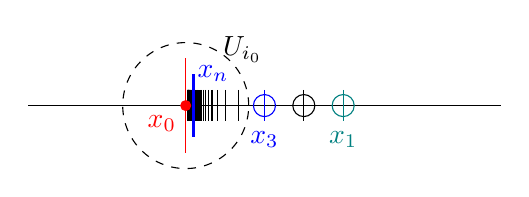
\begin{tikzpicture}[scale=2]
            % Dibuja el eje X
            \draw (-1,0) -- (2,0);

            % Dibuja los puntos 1/n
            \draw[teal] (1,0.1) -- (1,-0.1) node [below] {$x_{1}$};
            \draw[, teal] (1,0) circle (0.07cm);

            \draw (0.75,0.1) -- (0.75,-0.1);
            \draw[] (0.75,0) circle (0.07cm);

            \draw[blue] (1/2,0.1) -- (1/2,-0.1) node [below] {$x_{3}$};
            \draw[blue] (1/2,0) circle (0.07cm);

            \foreach \n in {3,4,...,80} {
                \draw (1/\n,0.1) -- (1/\n,-0.1);
            }
            \draw[blue, thick] (1/20,0.2) -- node [above, xshift=7pt, yshift=5pt] {$x_{n}$} (1/20,-0.2);
            
            % Dibuja el origen
            \draw[red] (0,0.3) -- (0,-0.3);

            % Dibuja el punto x_0
            \fill[red] (0,0) circle (1pt) node [below left] {$x_{0}$};

            % Dibuja un círculo centrado en el x_0
            \draw[dashed] (0,0) circle (0.4cm) node [above right, xshift=0.35cm, yshift=0.42cm] {$U_{i_0}$};
        \end{tikzpicture}
        \caption{Representación gráfica de los elementos de la demostración.}
    \end{figure}

    Sea $\{U_i\}_{i\in I}$, $U_i\in \T~\forall i\in I$ un recubrimiento de $A$ por abiertos de $X$. Entonces, como $x_0\in A$, $\exists i_0\in I$ tal que $x_0\in U_{i_0}$.
    Como $U_{i_0}\in \T$ con $x_0\in U_{i_0}$, tenemos que $U_{i_0}\in N_{x_0}$. Por tanto, como la sucesión converge a $x_0$, tenemos que
    $\exists n_0\in \bb{N}$ tal que $x_n\in U_{i_0}~\forall n\geq n_0$.

    Veamos qué ocurre con los $x_n$ con $n<n_0$. Como $\{U_i\}_{i\in I}$ es un recubrimiento de $A$, entonces para cada $n\in \bb{N},~n<n_0$, $\exists i_n\in I$ tal que $x_n\in U_{i_n}$.
    Por tanto, el subrecubrimiento finito es:
    \begin{equation*}
        \{U_{i_0}\} \cup \{U_{i_n}\}_{n=1,\dots,n_0-1}
    \end{equation*}

    Por tanto, $A$ es compacto.
\end{ejemplo}


Al igual que ocurría con la conexión, la compacidad se mantiene por funciones continuas:
\begin{samepage}
\begin{prop}
    Sea $f:(X,\T)\to (Y,\T')$ una aplicación continua entre espacios topológicos. Entonces:
    \begin{center}
        $X$ compacto $\Longrightarrow$ $f(X)$ compacto.
    \end{center}
\end{prop}
\end{samepage}
\begin{proof}
    Sea $\{U_i'\}_{i\in I}$, $U_i'\in \T'$ un recubrimiento de $f(X)$ por abiertos de $\T'$.

    Por la continuidad de $f$, $\forall i\in I$, $f^{-1}(U_i')\in \T$. Veamos que $\{f^{-1}(U_i')\}_{i\in I}$ es un recubrimiento de $X$ por abiertos de $\T$:
    \begin{equation*}
        X \subset f^{-1}(f(X)) \subset f^{-1}\left(\bigcup_{i\in I}U_i'\right) = \bigcup_{i\in I}f^{-1}(U_i') \subset X
    \end{equation*}

    Por ser $X$ compacto, $\exists I_0\subset I$ finito tal que $X=\bigcup\limits_{i\in I_0}f^{-1}(U_i')$. Por tanto,
    \begin{equation*}
        f(X) = f\left(\bigcup_{i\in I_0}f^{-1}(U_i')\right) = \bigcup_{i\in I_0}f(f^{-1}(U_i')) \subset \bigcup_{i\in I_0}U_i'
    \end{equation*}
    Por tanto, $\{U_i'\}_{i\in I_0}$ es un subrecubrimiento finito de $f(X)$ por abiertos de $\T'$, por lo que $f(X)$ es compacto.
\end{proof}
\begin{coro}
    La compacidad es una propiedad topológica.

    Es decir, si $f:(X,\T)\to (Y,\T')$ es un homeomorfismo, entonces $X$ es compacto si y solo si $f(X)=Y$ es compacto.
\end{coro}

Para el caso de los cocientes, tenemos el siguiente resultado:
\begin{prop}
    Sea $(X,\T)$ un espacio topológico, y sea $\cc{R}$ una relación de equivalencia en $X$. Consideramos $X/\cc{R}$ el espacio cociente con la topología cociente.
    Entonces:
    \begin{center}
        $X$ compacto $\Longrightarrow$ $X/\cc{R}$ compacto.
    \end{center}
\end{prop}
\begin{proof}
    Consideramos $p:(X,\T)\to (X/\cc{R}, \T/\cc{R})$ la proyección canónica en el cociente.
    Entonces, por el teorema anterior, como $p$ es continua, $p(X)$ es compacto. Pero como $p(X)=X/\cc{R}$ por ser $p$ sobreyectiva, entonces $X/\cc{R}$ es compacto.
\end{proof}

Para poder introducir ejemplos de aplicación de este teorema, incluimos antes el siguiente teorema.
Se generalizará más adelante en el Corolario de Heine-Borel (Corolario \ref{coro:HeineBorel}), aunque para demostrar este último emplearemos este caso particular:
\begin{teo}\label{teo:IntervaloRCompacto}
    Sea $(\bb{R},\T_u)$, y sea $a,b\in \bb{R}$ con $a<b$. Entonces, $[a,b]$ es compacto.
\end{teo}
\begin{proof}
    Sea $A=[a,b]$. Consideramos un recubrimiento de $A$ por abiertos de $\bb{R}$, $\{U_i\}_{i\in I}$, $U_i\in \T_u~\forall i\in I$.
    \begin{equation*}
        A\subset \bigcup_{i\in I}U_i \qquad \text{ con } U_i\in \T_u~\forall i\in I
    \end{equation*}

    Definimos el conjunto:
    \begin{equation*}
        J = \left\{x\in [a,b]\mid \exists I_0\subset I \text{ finito tal que } [a,x]\subset \bigcup_{i\in I_0}U_i\right\}
    \end{equation*}

    Para ver que $J$ es cerrado, basta con ver que $b\in J$.

    En primer lugar vemos que $J\neq \emptyset$. Como $a\in [a,b]$, $\exists i_0\in I$ tal que $a\in U_{i_0}$. Por tanto, $[a,a]\subset U_{i_0}$, por lo que $a\in J$.
    Además, si $x\in J$, entonces $[a,x]\subset J\subset [a,b]$, ya que, para todo $y\in [a,x]$, el mismo conjunto finito $I_0$ empleado para ver que $x\in J$ sirve para ver que $y\in J$, ya que
    $[a,y]\subset[a,x]\subset \bigcup\limits_{i\in I_0}U_i$. Por tanto,
    \begin{equation*}
        J = \begin{cases}
            [a,c[ \\
            ~~\lor \\
            [a,c]
        \end{cases} \text{ para un cierto } c\in [a,b]
    \end{equation*}

    Veamos ahora que el caso $J=[a,c[$ no es posible. Para ello, veamos que $c\in J$. Como $c\in [a,b]$, $\exists i_0\in I$ tal que $c\in U_{i_0}$.
    Como $c\in U_{i_0}\in \T_u$, entonces $\exists \varepsilon\in \bb{R}^+$ tal que $B(c,\varepsilon)=]c-\veps,c+\veps[\subset U_{i_0}$.
    Además, podemos suponer sin pérdida de generalidad que $x\in ]c-\veps, c[\subset J$, ya que en caso contrario tomamos un $\veps'$ menor de forma que se cumpla.
    Entonces, $\exists I_1\subset I$ finito tal que $[a,x]\subset \bigcup\limits_{i\in I_1}U_i$. Por tanto,
    \begin{equation*}
        [a,c] = [a,x]\cup [x,c] \subset \left(\bigcup_{i\in I_1}U_i\right) \cup ]c-\veps,c+\veps[ \subset \bigcup_{i\in I_1}U_i \cup U_{i_0}
    \end{equation*}
    Definiendo $I_2=I_1\cup \{i_0\}$, tenemos que $[a,c]\subset \bigcup\limits_{i\in I_2}U_i$, por lo que $c\in J$.

    Por tanto, $J=[a,c]$, para un cierto $c\in [a,b]$. Veamos ahora que $c=b$. Por reducción al absurdo, Supongamos que $c<b$.
    Como $c\in J$, $\exists I_0\subset I$ finito tal que $[a,c]\subset \bigcup\limits_{i\in I_0}U_i$.
    Además, como $c\in [a,b] \subset \bigcup\limits_{i\in I}U_i$, entonces $\exists i_0\in I$ tal que $c\in U_{i_0}$. Como $c\in U_{i_0}\in \T_u$,
    entonces $\exists \varepsilon\in \bb{R}^+$ tal que $B(c,\varepsilon)=]c-\veps,c+\veps[\subset U_{i_0}$. Definimos ahora $\veps' = \min\{\veps, b-c\}> 0$. Entonces,
    \begin{equation*}
        [a, c+\veps'[ = [a,c]\cup [c,c+\veps'[ \subset [a,c]\cup [c,c+\veps[ \subset
        \left(\bigcup_{i\in I_0}U_i\right) \cup ]c-\veps,c+\veps[ \subset \bigcup_{i\in I_0}U_i \cup U_{i_0}
    \end{equation*}
    Definiendo $I_1=I_0\cup \{i_0\}$, tenemos que $[a,c+\veps'[\subset \bigcup\limits_{i\in I_1}U_i$.
    Por tanto, $c+\dfrac{\veps'}{2}\in J$, llegando a una contradicción, ya que $J=[a,c]$. Por tanto, $c=b$.

    Por tanto, $J=[a,b]$. En particular, $b\in J$, por lo que $\exists I_0\subset I$ finito tal que $[a,b]\subset \bigcup\limits_{i\in I_0}U_i$.
    Es decir, $\{U_i\}_{i\in I_0}$ es un subrecubrimiento finito de $A$ por abiertos de $\bb{R}$, por lo que $A$ es compacto.    
\end{proof}

Una vez visto que $[a,b]$ es compacto, podemos ver el siguiente ejemplo de aplicación de que la compacidad se mantiene por funciones continuas:
\begin{ejemplo}
    Veamos que la circunferencia $\bb{S}^1$ es compacta. Consideramos la aplicación:
    \Func{f}{[0,1]}{\bb{S}^1}{x}{(\cos(2\pi x),\sen(2\pi x))}

    Tenemos que $f$ es continua y sobreyectiva. Por tanto, como $[0,1]$ es compacto, $\bb{S}^1=f([0,1])$ es compacto.
\end{ejemplo}



La compacidad por norma general no es hereditaria, pero sí se hereda a subconjuntos cerrados, como indica la siguiente proposición:
\begin{prop}\label{prop:CerradoCompacto}
    Sea $(X,\T)$ un espacio topológico compacto, y sea $C\subset X$. Entonces:
    \begin{center}
        $C\in C_\T$ cerrado $\Longrightarrow$ $C$ compacto.
    \end{center}
\end{prop}
\begin{proof}
    Sea $\{U_i\}_{i\in I}$, $U_i\in \T~\forall i\in I$ un recubrimiento mediante abiertos de $\T$ de $C$. Es decir, $$C\subset \bigcup\limits_{i\in I}U_i$$

    Entonces, $\{U_i\}_{i\in I}\cup \{X\setminus C\}$ es un recubrimiento de $X$ por abiertos de $\T$. Por ser $(X,\T)$ compacto, $\exists I_0\subset I$ finito tal que
    $\{U_i\}_{i\in I_0}\cup \{X\setminus C\}$ es un subrecubrimiento de $X$. Veamos que $\{U_i\}_{i\in I_0}$ es un sobrerecubrimiento finito de $C$ por abiertos de $\T$:
    \begin{align*}
        X = \left(\bigcup_{i\in I_0}U_i\right) \cup (X\setminus C) \Longrightarrow
        C &= C\cap X = C\cap \left(\left(\bigcup_{i\in I_0}U_i\right) \cup (X\setminus C)\right) =\\
        &= C\cap \left(\bigcup_{i\in I_0}U_i \right)
        \Longrightarrow C \subset \bigcup_{i\in I_0}U_i
    \end{align*}

    Por tanto, $C$ es compacto.
\end{proof}

Por tanto, se ha demostrado que ``cerrado implica compacto''\footnote{En realidad, no se ha demostrado exactamente eso.
Se ha demostrado que un subconjunto cerrado de un compacto es un compacto. Además, la proposición siguiente no es exactamente el
recíproco, ya que las hipótesis cambian. No obstante, debido a la similitud de los resultados, se expresa
como el recíproco para facilitar la interpretación.}. No obstante, para el recíproco necesitamos que el espacio topológico sea de Hausdorff:
\begin{prop}\label{prop:CompactoCerradoHausdorff}
    Sea $(X,\T)$ un espacio topológico de \ul{Hausdorff (T2)}, y sea $C\subset~X$. Entonces:
    \begin{center}
        $C$ compacto $\Longrightarrow$ $C\in C_\T$ cerrado.
    \end{center}
\end{prop}
\begin{proof}
    Probemos que $X\setminus C\in \T$. Fijamos $x_0\in X\setminus C$ y, para todo $x\in C$, como $X$ es T2 y $x\neq x_0$,
    $\exists U_x, \wt{U}_x\in \T$ tales que $x\in U_x$, $x_0\in \wt{U}_x$ y $U_x\cap \wt{U}_x=\emptyset$.

    Entonces, veamos que $\{U_x\}_{x\in C}$ es un recubrimiento de $C$ por abiertos de $\T$:
    \begin{equation*}
        C= \bigcup_{x\in C}\{x\} \subset \bigcup_{x\in C}U_x
    \end{equation*}


    Por ser $C$ compacto, $\exists n_0\in \bb{N}$ tal que $\{U_{x_n}\}_{\substack{n\in \bb{N}\\n\leq n_0}}$ es un subrecubrimiento finito de $C$ por abiertos de $\T$.

    Consideramos ahora $\wt{U}_{x_0}=\bigcap\limits_{n=1}^{n_0}\wt{U}_{x_n}$. Tenemos que $\wt{U}_{x_0}\in \T$ por ser intersección finita de abiertos de $\T$. Además, $x_0\in \wt{U}_{x_0}$.
    Veamos que $\wt{U}_{x_0}\cap C=\emptyset$. Para ello, vemos que:
    \begin{equation*}
        \wt{U}_{x_0}\cap U_{x_n} = \left(\bigcap\limits_{n=1}^{n_0}\wt{U}_{x_n}\right) \cap U_{x_n} \subset \wt{U}_{x_n}\cap U_{x_n} = \emptyset \hspace{1cm}
        \forall n\in \bb{N},~n\leq n_0
    \end{equation*}
    Por tanto,
    \begin{equation*}
        \wt{U}_{x_0}\cap C \subset \wt{U}_{x_0}\cap \left(\bigcup_{\substack{n\in \bb{N}\\n\leq n_0}}U_{x_n}\right) = \bigcup_{\substack{n\in \bb{N}\\n\leq n_0}}(\wt{U}_{x_0}\cap U_{x_n}) = \emptyset
    \end{equation*}

    Por tanto, tenemos que $x_0\in \wt{U}_{x_0}\subset X\setminus C$, con $\wt{U}_{x_0}\in \T$. Por tanto, $x_0\in [X\setminus C]^\circ$.
    Como $x_0\in X\setminus C$ es arbitrario, entonces $X\setminus C=[X\setminus C]^\circ$, por lo que $X\setminus C\in \T$ es abierto; es decir, $C$ es cerrado.
\end{proof}

Quitando la hipótesis de que el espacio topológico sea de Hausdorff, no es cierto que todo compacto sea cerrado, como muestra
el siguiente ejemplo:
\begin{ejemplo}
    Consideramos $\bb{R}$ con la topología cofinita $\T_{CF}$.
    Entonces, $\bb{R}\setminus \{0\}$ no es cerrado, ya que no es finito. No obstante, es fácil ver que es
    compacto de una forma similar a como se demostró que $(\bb{R},\T_{CF})$ es compacto.
\end{ejemplo}

Como consecuencia de las dos proposiciones anteriores, se tiene el siguiente corolario, el cual no es trivial, respecto de la intersección de compactos.
\begin{coro} \label{coro:InterseccionCompactos}
    Sea $(X,\T)$ un espacio topológico de Hausdorff (T2). Sea $\{A_i\}_{i\in I}$, $A_i\subset X$ una familia de compactos de $X$.
    Entonces:
    \begin{center}
        $\bigcap\limits_{i\in I}A_i$ compacto.
    \end{center}
\end{coro}
\begin{proof}
    Sea $A=\bigcap\limits_{i\in I}A_i$. Como $A_i$ es compacto $\forall i\in I$ y $(X,\T)$ es T2, entonces $A_i\in C_\T$ cerrado $\forall i\in I$ por la proposición \ref{prop:CompactoCerradoHausdorff}.
    Además, como la intersección arbitraria de cerrados es cerrada, entonces $A\in C_\T$ cerrado.

    Fijado $i\in I$, como $A\subset A_i$ es un subconjunto cerrado de un compacto $(A_i)$, entonces $A$ es compacto por la proposición \ref{prop:CerradoCompacto}.
\end{proof}

Para la unión de compactos, tenemos el siguiente resultado, más general que el anterior ya que no se impone nada sobre $(X,\T)$:
\begin{prop} \label{prop:UnionCompactos}
    Sea $(X,\T)$ un espacio topológico. Entonces:
    \begin{center}
        $A,B\subset X$ compactos $\Longrightarrow A\cup B$ compacto.
    \end{center}
\end{prop}
\begin{proof}
    Sea $\{U_i\}_{i\in I}$, $U_i\in \T$ un recubrimiento de $A\cup B$ por abiertos de $\T$, es decir,
    \begin{equation*}
        A\cup B \subset \bigcup_{i\in I}U_i
    \end{equation*}

    Como $A\subset A\cup B$, entonces $\{U_i\}_{i\in I}$ es un recubrimiento de $A$ por abiertos de $\T$, y como $A$ es compacto, $\exists I_A\subset I$ finito tal que $\{U_i\}_{i\in I_A}$ es un subrecubrimiento finito de $A$,
    es decir,
    \begin{equation*}
        A \subset \bigcup_{i\in I_A}U_i
    \end{equation*}

    Análogamente, como $B\subset A\cup B$, entonces $\{U_i\}_{i\in I}$ es un recubrimiento de $B$ por abiertos de $\T$, y como $B$ es compacto, $\exists I_B\subset I$ finito tal que $\{U_i\}_{i\in I_B}$ es un subrecubrimiento finito de $B$,
    es decir,
    \begin{equation*}
        B \subset \bigcup_{i\in I_B}U_i
    \end{equation*}

    Por tanto, $\{U_i\}_{i\in I_A\cup I_B}$ es un subrecubrimiento de $A\cup B$ por abiertos de $\T$:
    \begin{equation*}
        A\cup B \subset \left(\bigcup_{i\in I_A}U_i\right) ~\bigcup~ \left(\bigcup_{i\in I_B}U_i\right) = \bigcup_{i\in I_A\cup I_B}U_i
    \end{equation*}

    Como $I_A\cup I_B$ es finito, entonces dicho subrecubrimiento es finito, por lo que $A\cup B$ es compacto.
\end{proof}


Veamos el siguiente ejemplo de aplicación de esta proposición:
\begin{ejemplo}
    Veamos si $(\bb{R},\T_{CF})$ es T2.
    
    Consideramos $A=[0,+\infty[$, que claramente no es cerrado. Además, es fácil demostrar que es compacto (se demuestra de forma análoga a que $(\bb{R},\T_{CF})$ lo es).
    Por tanto, como $A\subset \bb{R}$ es compacto pero no cerrado, tenemos que $(\bb{R},\T_{CF})$ no es T2, como ya se demostró en el el apartado \ref{ex:T_CF_T1noT2} del ejemplo de la página \pageref{ex:T_CF_T1noT2}.
\end{ejemplo}


El siguiente resultado nos será de gran utilidad para demostrar que una aplicación es cerrada:
\begin{teo}\label{teo:ContinuaEntoncesCerrada}
    Sea $(X,\T)$ un espacio topológico compacto y $(Y,\T')$ un espacio topológico de Hausdorff (T2).
    Entonces, toda aplicación $f:(X,\T)\to (Y,\T')$ continua es cerrada.
\end{teo}
\begin{proof}
    Sea $C\subset X$ un subconjunto cerrado de $X$. Tenemos que ver que $f(C)$ es cerrado en $Y$.
    
    Como $C\subset X$ es cerrado y $X$ es compacto, entonces $C$ es compacto por la Proposición \ref{prop:CerradoCompacto}.
    Como $f$ es continua y $C$ es compacto, entonces $f(C)$ es compacto. Por tanto, como $Y$ es de T2, $f(C)$ es cerrado.
\end{proof}


Por último, tenemos el siguiente resultado, que nos sirve para estudiar la compacidad de productos de espacios topológicos:
\begin{teo}[Tychonoff\footnote{También escrito como Tijonov, Tychonov.}] \label{teo:Tychonoff}
    Sean $(X,\T)$ e $(Y,\T')$ dos espacios topológicos. Entonces,
    \begin{center}
        $X$ e $Y$ compactos $\Longrightarrow$ $X\times Y$ compacto.
    \end{center}
\end{teo}
\begin{proof}
    Demostramos por doble implicación:
    \begin{description}
        \item[$\Longleftarrow)$] Como $X\times Y$ es compacto y la proyección en $X$, $\pi_X$ es continua, entonces $(X\times Y)=X$ es compacto.
        Análogamente, se demuestra que $Y$ es compacto.
        
        \item[$\Longrightarrow)$] % // TODO: Completar Producto de compactos es compacto
        
        Supongamos que $X$ e $Y$ son compactos.
        
        \begin{comment}
        Demostraremos que todo recubrimiento de $X\times Y$ por abiertos básicos de $\T\times \T'$
        tiene un subrecubrimiento finito. Para ello, sea \{$U_i\times V_i$\}$_{i\in I}$ un recubrimiento de $X\times Y$ por abiertos básicos de $\T\times \T'$,
        es decir, $U_i\in \T$, $V_i\in \T'$ $\forall i\in I$ y:
        \begin{equation*}
            X\times Y = \bigcup_{i\in I}U_i\times V_i
        \end{equation*}
        \end{comment}
    \end{description}
\end{proof}


\subsection{Compacidad en espacios métricos}

\begin{definicion}[Conjunto acotado]
    Sea $(X,d)$ un espacio métrico. Decimos que $A\subset X$ es acotado si $\exists x_0\in X$ y $r\in \bb{R}^+$ tal que $A\subset B(x_0,r)$.
\end{definicion}
\begin{lema}
    Sea $(X,d)$ un espacio métrico. Entonces, $A\subset X$ es acotado si y solo si, para cada $x\in X$, $\exists r_x\in \bb{R}^+$ tal que $A\subset B(x,r_x)$.
\end{lema}
\begin{proof}
    Demostramos por doble implicación:
    \begin{description}
        \item[$\Longleftarrow)$] Se tiene de forma directa.
        \item[$\Longrightarrow)$] Como $A$ es acotado, $\exists x_0\in X$ y $r'\in \bb{R}^+$ tal que $A\subset B(x_0,r')$. Para cada $x\in X$, consideramos $r_x=d(x,x_0)+r'$.
        Veamos que $A\subset B(x,r)$. Sea $y\in A$. Entonces:
        \begin{equation*}
            d(y,x) \leq d(y,x_0) + d(x_0,x) < r' + d(x_0,x) = r_x \Longrightarrow y\in B(x,r_x)  
        \end{equation*}
        Por tanto, $A\subset B(x,r_x)$.  \qedhere
    \end{description}
\end{proof}


Una vez introducido el concepto de conjunto acotado, tenemos el siguiente resultado:
\begin{prop}\label{prop:CompactoCerradoAcotado}
    Sea $(X,d)$ un espacio métrico, y sea $A\subset X$. Tenemos que:
    \begin{center}
        $A$ es compacto $\Longrightarrow$ $A$ es cerrado y acotado.
    \end{center}
\end{prop}
\begin{proof}
    Como $A$ es compacto, por ser $(X,d)$ T2 (ver Lema \ref{lema:Metrizable}), por la Proposición \ref{prop:CompactoCerradoHausdorff} tenemos que $A$ es cerrado. Veamos ahora que está acotado.
        
    Como las bolas abiertas son abiertos de $X$, fijado $x_0\in X$ tomamos el siguiente recubrimiento de $A$ por abiertos de $X$:
    \begin{equation*}
        A\subset X = \bigcup_{n \in \bb{N}}B(x_0,n)
    \end{equation*}

    Por ser $A$ compacto, $\exists n_1,\dots,n_k\in \bb{N}$ tal que $A\subset \bigcup\limits_{i=1}^k B(x_0,n_i)$.
    Tomando $r=\max\{n_1,\dots,n_k\}$ conjunto finito, tenemos que $$A\subset \bigcup\limits_{i=1}^k B(x_0,n_i) \subset B(x_0,r).$$
    
    Por tanto, $A$ es acotado.
\end{proof}

\begin{coro}[Heine-Borel] \label{coro:HeineBorel}
    Sea $(\bb{R}^n,\T_u)$, y consideramos $A\subset \bb{R}^n$. Entonces:
    \begin{center}
        $A$ es compacto $\Longleftrightarrow$ $A$ es cerrado y acotado.
    \end{center}
\end{coro}
\begin{proof}
    Demostramos por doble implicación:
    \begin{description}
        \item[$\Longrightarrow)$] Esto se ha demostrado en la Proposición \ref{prop:CompactoCerradoAcotado} para cualquier espacio métrico.
        \item[$\Longleftarrow)$] Como $A$ es acotado, tenemos que $\exists R\in \bb{R}^+$ tal que $A\subset B(0,R)\subset \ol{B}(0,R)$. Sea $x=(x_1,\dots,x_n)\in A$.
        Entonces, como $\|x\|\leq R$, tenemos que $|x_i|\leq R$ $\forall i=1,\dots,n$; es decir, $A$ está acotado coordenada a coordenada. Por tanto,
        \begin{equation*}
            A\subset [-R,R]^n = [-R,R] \times \overbrace{\cdots}^{(n)} \times [-R,R]
        \end{equation*}

        Tenemos que $[-R,R]$ es compacto por ser un intervalo cerrado y acotado (Teorema \ref{teo:IntervaloRCompacto}).
        Además, por el Teorema de Tychonoff (Teorema \ref{teo:Tychonoff}), $[-R,R]^n$ es compacto.
        Por tanto, $A$ es un subconjunto cerrado de un compacto, por lo que $A$ es compacto (Proposición \ref{prop:CerradoCompacto}).
    \end{description}
\end{proof}

\begin{ejemplo}
    Algunos ejemplos de conjuntos compactos son:
    \begin{enumerate}
        \item La esfera $\bb{S}^{n}$ es compacta.
        \item El toro es compacto por ser homeomorfo a $(\bb{S}^1\times \bb{S}^1)/\cc{R}$, y este lo es por serlo $\bb{S}^1\times \bb{S}^1$, que es producto de compactos.
    \end{enumerate}
\end{ejemplo}

Como corolario al Corolario de Heine-Borel, tenemos el siguiente resultado:
\begin{coro}
    Sea $(X,\T)$ un espacio topológico compacto y sea la aplicación $f:(X,\T)\to (\bb{R},\T_u)$ continua.    
    Entonces, $f$ es acotada (alcanza un máximo y un mínimo absolutos). Es decir,
    \begin{equation*}
        \exists x_0,x_1\in X \mid f(x_0) \leq f(x) \leq f(x_1) \hspace{1cm} \forall x\in X
    \end{equation*}
\end{coro}
\begin{proof}
    Como $f$ es continua y $X$ es compacto, entonces $f(X)\subset \bb{R}$ es compacto. Por tanto, $f(X)$ es cerrado y acotado.

    Por ser $f(X)$ acotada, $f(X)$ está mayorada y minorada, y por el Axioma del Supremo $\exists i=\inf f(X)$, $s=\sup f(X)$. Además, sabemos que:
    \begin{equation*}
        i\in \ol{f(X)}\AstIg f(X) \hspace{1cm}
        s\in \ol{f(X)}\AstIg f(X)
    \end{equation*}
    donde en $(\ast)$ hemos empleado que $f(X)$ es cerrado. Por tanto, el ínfimo y el supremo están en $f(X)$, por lo que son mínimo y máximo respectivamente.
    Además, $\exists x_0,x_1\in X$ tales que $f(x_0)=i$ y $f(x_1)=s$.

    %// TODO: Ver por qué ínfimo y supremo están en la adherencia
\end{proof}


\section{Relación de Ejercicios}
Para ver ejercicios relacionados con el Tema 3, consultar la sección \ref{sec:Rel3}.